%____________________________________________________________________________||
\section{Interpretation in Dark Matter models} \label{sec:darkmatter}

In Run~1, the results of the \alphat analysis were interpreted in the context of
supersymmetric simplified models. For Run~2, significant effort has been invested
in extending the analysis strategy to include searches for the production of dark
matter, namely the inclusion of the asymmetric and monojet categories.

The generic signature of dark matter pair production in colliders is missing
transverse momentum from the dark matter along with recoiling energetic visible
particles that are used to trigger the event. First analyses used contact 
operators~\cite{Goodman:2010ku} in effective field theories (EFTs) with various 
coupling structures to interpret dark matter searches. Experimental limits using
monojet final states have been published using 7 and 8 TeV LHC 
data~\cite{Chatrchyan:2012me,ATLAS:2012ky} for a variety of operators.

%In addition, similar final states with the form $\chi \bar \chi + X$, where
%$\chi$ is the dark matter particle and $X$ can be a photon, jet, or other
%particle, have been studied in the context of effective operators These
%additional particles are initial state radiation (ISR) radiated off from the
%interacting partons. (e.g.
%\cite{Goodman:2010yf,Fox:2011pm,Petriello:2008pu,Fox:2011fx}).

The lack of predictive information and severe validity constraints of EFTs have
lead to the development of improved minimal simplified dark matter (MSDM) models.
These models enable the comparison between different experimental
searches in a relatively model-independent way~\cite{Buchmueller:2014yoa}.

%Previous CMS analyses performed the search for new physics in the monojet final
%state, as detailed in References~\cite{Aad:2011xw, ATLAS:2012ky} using up to
%$4.7\,\fbi$ of data with proton-proton collision at a center-of-mass energy of
%$\sqrt{s}=7\,\tev$. A conference note~\cite{ATLAS-CONF-2012-147} using
%8$\,\tev$ data has also been published, based on half of the 2012 dataset. 


%The present document also describes the planned analysis of WIMP pair
%production in association with light and heavy quarks using the upcoming 13~TeV
%data set corresponding.  Hadronic final states of the form $\chi \bar \chi +
%X$, where $\chi$ is the dark matter particle and $X$ can be one or several jets
%have been studied in the context of effective operators. These jets are either
%directly produced due in the interaction between SM and DM or are initial state
%radiation (ISR)  radiated off from the interacting partons (e.g.
%\cite{Goodman:2010yf,Fox:2011pm,Petriello:2008pu,Fox:2011fx}). As detailed in
%Ref.~\cite{Lin:2013sca, Artoni:2013zba} particular the use of heavy quarks,
%namely $b$- and top quarks take advantage of quark-mass dependency of scalar
%couplings. The quark mass dependency comes from minimal flavor violation
%assumptions. Further advantages gained by the use of third generation quarks is
%to extend the analysis to larger jet multiplicities and therefore larger signal
%acceptance compared to the monojet analysis. Thus accessing a unique and
%orthogonal phase space. 


%This analysis will also set strongest constraints for low mass dark matter, and
%the strongest collider constraints across a wide range of masses. We will also
%start to probe excesses observed in direct detection experiment at energies of
%about 10 GeV in the DAMA (2008), CoGent (2010/11), CREST-II (2012) and CDMS
%(2013) experiments but also by the Fermi-LAT (2013) satellite indicating a DM
%particle of about 50 GeV mass. We expect to place stringent constraints on this
%phase space in the near future with the $13$~TeV run.

The \alphat analysis is sensitive to DM production in association with both
light ($g,~u,~d,~c,~s$) and heavy flavoured ($b,~t$) jets. In this section we
present the expected sensitivity of the analysis to these topologies with 2~\ifb
of 13 TeV data. The simplified models considered in the interpretations are those
recommended by the ATLAS-CMS DM Forum for early LHC Run~2 searches. We have
utilised all available Spring15 samples of the corresponding models that were
available at the time of writing. These samples populate key regions of the
{\mphi-\mchi} mass plane, and correspond roughly to those shown in
Tab.~\ref{tab:DMgrid}.

\begin{table}[h!] \centering \begin{tabular}{l|llllllllll}\hline \hline
$m_\textrm{DM}$  & \multicolumn{10}{c}{$m_\Phi$}
\\ \hline 1    & 10 & 20 & 50 & 100 & 200 & 300 & 500 & 1000 & 2000 & 10000 \\
10   & 10 & 15 & 50 & 100 &     &     &     &      &      & 10000 \\ 50   & 10 &
& 50 & 95  & 200 & 300 &     &      &      & 10000 \\ 150  & 10 &    &    &
& 200 & 295 & 500 & 1000 &      & 10000 \\ 500  & 10 &    &    &     &     &
& 500 & 995  &      & 10000 \\ 1000 & 10 &    &    &     &     &     &     &
1000 & 1995 & 10000\\ \hline \hline \end{tabular} \caption{Benchmark dark
matter and mediator masses. The parameter space follows the
DM Forum recommendations~\cite{Abercrombie:2015wmb}. Points are chosen roughly
equidistant on a logarithmic scale. Points on the on-shell diagonal are always 
chosen to be 5 GeV away from the threshold to avoid numerical instabilities in 
the event generation.} \label{tab:DMgrid} \end{table}


%\subsection{Simplified Models}



\subsection{Light flavour models} \label{sec:dm_lightjet}

The light flavour simplified models consist of a DM particle \pchi of mass
\mchi that is a Diract fermion, and a spin-1 (vector or axial-vector) or spin-0
(scalar or pseudoscalar) mediating particle \pphi of mass \mphi in an
$s$-channel. The couplings of the mediator with the standard model and dark
matter particles are given by \gsm and \gdm, respectively. The recommendations
by the DM Forum on the choice of couplings is \gsm$=1$,\gdm$=1$ for
(pseudo)scalar models, and \gsm$=0.25$,\gdm$=1$ for (axial-)vector models.
Assuming that no additional visible or invisible particles contribute to the decay 
of the mediator, we impose the minimal width determined by the choice of couplings. 
An example Feynman diagram is shown in Fig.~\ref{fig:DMfeynman}.


%The primary simplified models for Dirac fermion DM studied and recommended by
%the ATLAS-CMS DM Forum for early LHC Run-2 searches are comprised of spin-0 and
%spin-1 mediators using $s$-channel and $t$-channel models.We consider the case
%of a DM particle $\chi$ of mass $m_{\chi}$ that is a Dirac fermion and where the
%production proceeds via the exchange of a spin-1 mediator $\Phi$ of mass
%$m_{\Phi}$ in the $s$-channel. Two models with vector (V) and axial-vector (AV)
%couplings are considered. The coupling to the standard model $g_{\textrm SM}$ is
%assumed to be universal for all quark families and $g_{\textrm DM}$ is the
%coupling to the dark matter particles. Assuming that no additional visible or
%invisible particles contribute to the decay we use the minimal width determined
%by the choice of $g_{\textrm SM}$ and $g_{\textrm DM}$ as shown in
%Fig.~\ref{fig:DMfeynman}.

\begin{figure}[h!] \centering
\subfigure{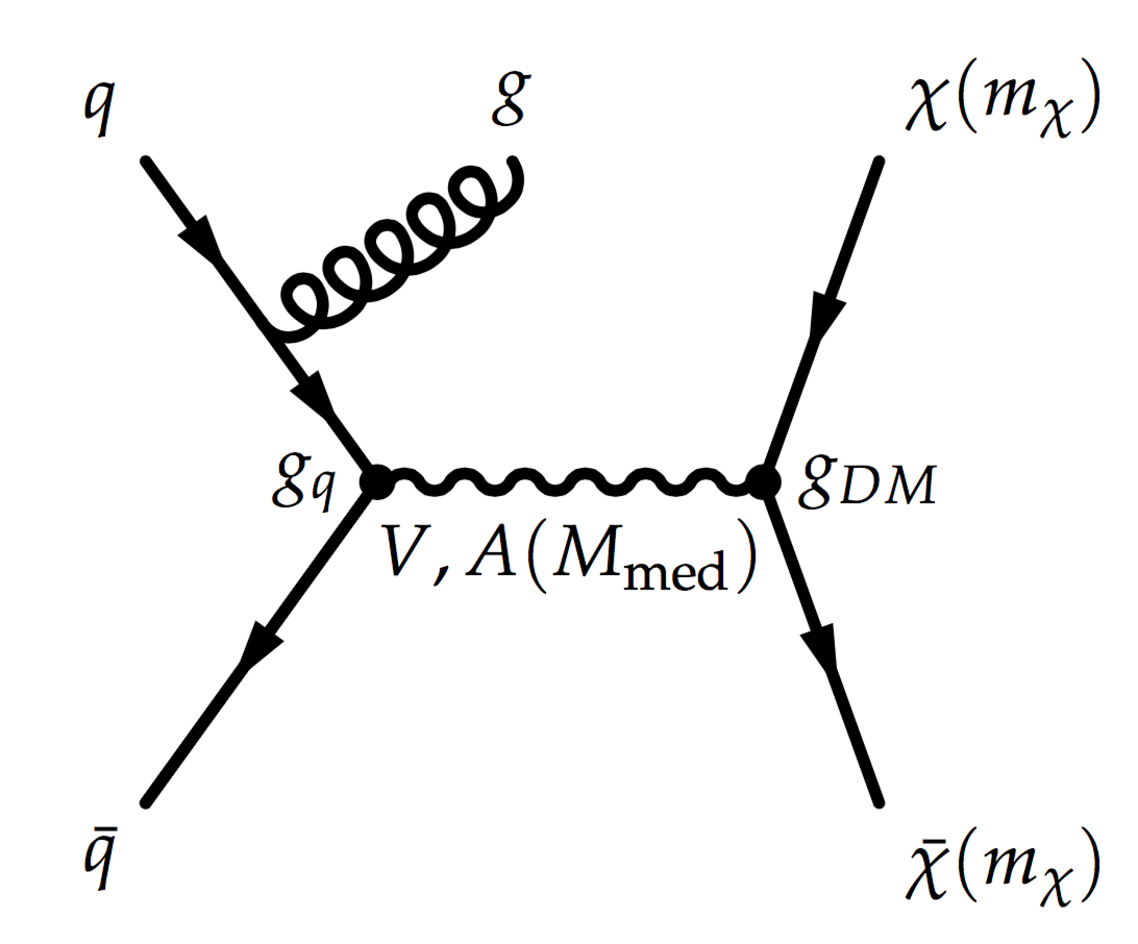
\includegraphics[width=0.35\textwidth]{figures/DMplots/feynman_light_jet.pdf}}
\caption{Representative Feynman diagram showing the pair production of Dark
Matter particles in association with a parton from the initial state via a
vector or axial-vector mediator. The cross section and kinematics depend upon
the mediator and Dark Matter masses, and the mediator couplings to Dark Matter
and quarks respectively: ($m_{\Phi} ,\ m_\textrm{DM} ,\, g_{\textrm DM} ,\,
g_{\textrm SM})$. \cite{Abercrombie:2015wmb}} \label{fig:DMfeynman} \end{figure}


%We consider four simplified models resulting in final states dominated by light
%quarks ($u,~d,~c,~s$) production. These models probe the axial-vector (A),
%vector (V), scalar (S) and pseudo-scalar (P) coupling of the mediator between
%dark matter and standard model particles. Currently the couplings constants
%$g_\textrm{DM}$ and $g_\textrm{SM}$ are assumed to be one. This document will be
%updated to reflect a recent recommendation of $g_\textrm{SM}=0.25$. We have used
%all the official CMS samples that were available at the time of writing.

Assuming 2~\ifb of data we list the cross sections, yields and selection 
efficiencies for the four light jet models in
Tables~\ref{tab:dm_V_g1_2fb}-\ref{tab:dm_P_g1_2fb}. The signal selection
efficiencies are around $\sim 1$\% for mass points near the expected exclusion
region, and are correspondingly larger (smaller) for higher (lower) mass points.
The asymmetric and monojet categories are seen to almost double the acceptance
to these models compared to the Run~1 symmetric categories alone, justifying the
inclusion of these selections into the analysis.

\clearpage 
\begin{table}
\renewcommand{\arraystretch}{1.0}
\small
\centering
\begin{tabular}{lllllll}
\hline
$m_\phi$ & $m_\chi$ & $\sigma$ [pb] & Yield (sym) & Yield (asy) & Yield (mon) & Efficiency [\%] \\ \hline
10000     &   100       &   2.51e-03  &   0.07      &   0.02      &   0.04      &   1.38      \\ 
10000     &   150       &   2.24e-03  &   0.07      &   0.02      &   0.04      &   1.56      \\ 
10000     &   50        &   2.84e-03  &   0.06      &   0.02      &   0.03      &   1.10      \\ 
1000      &   100       &   4.11e+01  &   1107.27   &   279.91    &   565.94    &   1.35      \\ 
1000      &   150       &   4.02e+01  &   1147.46   &   287.23    &   603.26    &   1.43      \\ 
1000      &   50        &   4.57e+01  &   1272.87   &   302.50    &   699.23    &   1.39      \\ 
100       &   100       &   1.19e+03  &   8588.02   &   2411.80   &   4604.37   &   0.36      \\ 
100       &   10        &   9.79e+04  &   87537.01  &   29383.31  &   40665.66  &   0.04      \\ 
100       &   50        &   2.96e+04  &   45100.19  &   13667.83  &   25859.11  &   0.08      \\ 
2000      &   100       &   2.70e+00  &   115.24    &   31.42     &   57.52     &   2.14      \\ 
200       &   100       &   3.71e+03  &   19511.17  &   4393.45   &   11959.69  &   0.26      \\ 
200       &   10        &   1.25e+04  &   48534.78  &   13502.52  &   25570.36  &   0.19      \\ 
200       &   150       &   4.18e+02  &   5561.86   &   1298.57   &   3156.65   &   0.67      \\ 
200       &   1         &   1.31e+04  &   56454.39  &   17681.43  &   28950.18  &   0.22      \\ 
200       &   50        &   1.09e+04  &   44088.03  &   11850.36  &   24632.48  &   0.20      \\ 
20        &   1         &   6.38e+06  &   72483.61  &   0.00      &   0.00      &   0.00      \\ 
300       &   100       &   2.44e+03  &   19720.73  &   4445.89   &   11576.49  &   0.40      \\ 
300       &   10        &   3.54e+03  &   29071.13  &   6856.89   &   16700.41  &   0.41      \\ 
300       &   150       &   9.46e+02  &   8744.02   &   2265.54   &   4810.24   &   0.46      \\ 
300       &   50        &   3.27e+03  &   26866.17  &   6843.17   &   14620.56  &   0.41      \\ 
500       &   100       &   4.86e+02  &   7380.17   &   1893.05   &   4192.51   &   0.76      \\ 
500       &   10        &   5.88e+02  &   9061.43   &   2347.71   &   4872.11   &   0.77      \\ 
500       &   150       &   3.98e+02  &   6360.90   &   1761.40   &   3418.34   &   0.80      \\ 
500       &   1         &   5.91e+02  &   10385.84  &   2800.08   &   5636.24   &   0.88      \\ 
500       &   50        &   5.42e+02  &   8462.85   &   2268.04   &   4672.87   &   0.78      \\ 
50        &   10        &   6.10e+05  &   47859.40  &   28684.06  &   14400.69  &   0.00      \\ 
50        &   1         &   6.61e+05  &   121202.87 &   34849.16  &   61463.90  &   0.01      \\ 
50        &   50        &   1.01e+04  &   28974.34  &   8068.27   &   14747.42  &   0.14      \\ 
\hline
\end{tabular}
\caption{Cross section, yields at 2 \ifb (split according to symmetric, asymmetric, and monojet categories), and total selection efficiency for the vector light jet samples.}
\label{tab:dm_V_g1_2fb}
\end{table}
 \clearpage
\begin{table}
\renewcommand{\arraystretch}{1.0}
\small
\centering
\begin{tabular}{lllllll}
\hline
$m_\phi$ & $m_\chi$ & $\sigma$ [pb] & Yield (sym) & Yield (asy) & Yield (mon) & Efficiency [\%] \\ \hline
10000     &   10        &   2.91e-03  &   0.07      &   0.02      &   0.04      &   1.17      \\ 
10000     &   1         &   2.88e-03  &   0.07      &   0.02      &   0.04      &   1.26      \\ 
10000     &   50        &   2.54e-03  &   0.08      &   0.02      &   0.04      &   1.49      \\ 
1000      &   10        &   4.83e+01  &   1178.17   &   289.85    &   629.83    &   1.22      \\ 
1000      &   1         &   4.95e+01  &   1142.25   &   289.22    &   594.70    &   1.15      \\ 
1000      &   50        &   4.46e+01  &   1131.30   &   264.21    &   618.53    &   1.27      \\ 
100       &   100       &   4.11e+02  &   4384.24   &   1050.68   &   2357.71   &   0.53      \\ 
100       &   1         &   1.00e+05  &   101995.59 &   36805.44  &   52340.20  &   0.05      \\ 
100       &   50        &   8.00e+03  &   23369.91  &   7118.13   &   12993.94  &   0.15      \\ 
2000      &   100       &   2.46e+00  &   79.13     &   21.02     &   41.54     &   1.61      \\ 
2000      &   150       &   2.10e+00  &   74.72     &   19.70     &   37.32     &   1.78      \\ 
2000      &   1         &   3.06e+00  &   92.42     &   22.76     &   49.06     &   1.51      \\ 
200       &   10        &   1.23e+04  &   51056.48  &   11985.12  &   29218.46  &   0.21      \\ 
200       &   1         &   1.31e+04  &   52831.74  &   14467.39  &   30866.86  &   0.20      \\ 
200       &   50        &   7.21e+03  &   35890.11  &   9161.42   &   19359.67  &   0.25      \\ 
20        &   10        &   4.58e+05  &   93914.10  &   12513.71  &   53173.72  &   0.01      \\ 
20        &   1         &   6.44e+06  &   103204.94 &   34447.50  &   68757.44  &   0.00      \\ 
300       &   100       &   1.22e+03  &   13105.43  &   3878.97   &   7016.05   &   0.54      \\ 
300       &   10        &   3.59e+03  &   27848.92  &   6970.75   &   15647.50  &   0.39      \\ 
300       &   150       &   2.49e+02  &   3286.71   &   842.69    &   1723.61   &   0.66      \\ 
300       &   1         &   3.68e+03  &   26982.67  &   6253.03   &   15556.70  &   0.37      \\ 
300       &   50        &   2.68e+03  &   25546.89  &   6264.67   &   14470.72  &   0.48      \\ 
500       &   100       &   3.83e+02  &   6791.40   &   1719.08   &   3706.41   &   0.89      \\ 
500       &   10        &   6.32e+02  &   8883.82   &   2245.14   &   5025.72   &   0.70      \\ 
500       &   150       &   2.41e+02  &   4093.84   &   1057.36   &   2238.78   &   0.85      \\ 
500       &   1         &   6.37e+02  &   8864.53   &   2393.54   &   4694.17   &   0.70      \\ 
500       &   50        &   5.32e+02  &   7954.51   &   2031.11   &   4428.90   &   0.75      \\ 
50        &   10        &   4.70e+05  &   111414.74 &   29186.42  &   71315.44  &   0.01      \\ 
50        &   1         &   6.79e+05  &   116310.63 &   15959.55  &   31470.40  &   0.01      \\ 
50        &   50        &   3.74e+03  &   13222.86  &   4101.89   &   7254.64   &   0.18      \\ 
\hline
\end{tabular}
\caption{Cross section, yields at 2~\ifb (split according to symmetric, asymmetric, and monojet categories), and total selection efficiency for the axial-vector light jet samples.}
\label{tab:dm_A_g1_2fb}
\end{table}
 \clearpage
\begin{table}
\renewcommand{\arraystretch}{1.0}
\footnotesize
\centering
\begin{tabular}{lllllll}
\hline
$m_\phi$ & $m_\chi$ & $\sigma$ [pb] & Yield (sym) & Yield (asy) & Yield (mon) & Efficiency [\%] \\ \hline
10000     &   1000      &   6.76e-09  &   0.00      &   0.00      &   0.00      &   2.37      \\ 
10000     &   10        &   2.34e-06  &   0.00      &   0.00      &   0.00      &   0.77      \\ 
10000     &   150       &   1.34e-06  &   0.00      &   0.00      &   0.00      &   0.96      \\ 
10000     &   1         &   2.36e-06  &   0.00      &   0.00      &   0.00      &   0.74      \\ 
10000     &   500       &   1.08e-07  &   0.00      &   0.00      &   0.00      &   1.86      \\ 
10000     &   50        &   2.18e-06  &   0.00      &   0.00      &   0.00      &   0.80      \\ 
1000      &   1000      &   1.62e-06  &   0.00      &   0.00      &   0.00      &   2.26      \\ 
1000      &   100       &   1.84e-01  &   4.12      &   1.31      &   1.63      &   1.12      \\ 
1000      &   10        &   1.93e-01  &   4.26      &   1.34      &   1.64      &   1.10      \\ 
1000      &   150       &   1.68e-01  &   3.64      &   1.15      &   1.40      &   1.08      \\ 
1000      &   1         &   1.97e-01  &   4.32      &   1.37      &   1.75      &   1.09      \\ 
1000      &   500       &   2.58e-03  &   0.07      &   0.02      &   0.03      &   1.34      \\ 
1000      &   50        &   1.94e-01  &   4.32      &   1.32      &   1.68      &   1.12      \\ 
100       &   100       &   3.30e-01  &   3.11      &   1.06      &   1.35      &   0.47      \\ 
100       &   10        &   1.14e+02  &   294.71    &   96.97     &   135.89    &   0.13      \\ 
100       &   1         &   1.14e+02  &   278.07    &   84.60     &   127.56    &   0.12      \\ 
100       &   50        &   2.04e+00  &   10.42     &   3.64      &   4.41      &   0.26      \\ 
10        &   10        &   9.95e+00  &   22.29     &   7.23      &   11.13     &   0.11      \\ 
10        &   1         &   1.16e+03  &   288.78    &   78.95     &   144.23    &   0.01      \\ 
2000      &   1000      &   1.99e-05  &   0.00      &   0.00      &   0.00      &   2.09      \\ 
2000      &   100       &   2.92e-03  &   0.09      &   0.03      &   0.03      &   1.47      \\ 
2000      &   10        &   3.26e-03  &   0.09      &   0.03      &   0.03      &   1.37      \\ 
2000      &   150       &   2.61e-03  &   0.08      &   0.02      &   0.03      &   1.50      \\ 
2000      &   1         &   3.27e-03  &   0.09      &   0.03      &   0.03      &   1.37      \\ 
2000      &   500       &   1.16e-03  &   0.04      &   0.01      &   0.02      &   1.92      \\ 
2000      &   50        &   3.17e-03  &   0.09      &   0.03      &   0.03      &   1.38      \\ 
200       &   100       &   8.18e-01  &   6.41      &   2.17      &   2.82      &   0.39      \\ 
200       &   10        &   3.95e+01  &   224.49    &   80.00     &   96.19     &   0.28      \\ 
200       &   150       &   1.70e-01  &   1.74      &   0.56      &   0.74      &   0.51      \\ 
200       &   1         &   3.18e+01  &   184.12    &   52.35     &   83.96     &   0.29      \\ 
200       &   50        &   3.95e+01  &   230.66    &   77.79     &   99.61     &   0.29      \\ 
20        &   10        &   1.21e+01  &   18.21     &   4.73      &   8.66      &   0.08      \\ 
20        &   1         &   7.18e+02  &   356.47    &   114.30    &   161.44    &   0.02      \\ 
300       &   100       &   2.32e+01  &   184.25    &   62.45     &   80.01     &   0.40      \\ 
300       &   10        &   2.32e+01  &   182.25    &   68.25     &   69.57     &   0.39      \\ 
300       &   150       &   4.86e-01  &   4.67      &   1.60      &   1.86      &   0.48      \\ 
300       &   1         &   2.32e+01  &   177.75    &   61.74     &   76.83     &   0.38      \\ 
300       &   50        &   2.32e+01  &   182.55    &   61.69     &   81.21     &   0.39      \\ 
5000      &   1000      &   3.29e-07  &   0.00      &   0.00      &   0.00      &   2.51      \\ 
5000      &   100       &   3.02e-05  &   0.00      &   0.00      &   0.00      &   0.92      \\ 
5000      &   10        &   3.94e-05  &   0.00      &   0.00      &   0.00      &   0.88      \\ 
5000      &   150       &   2.24e-05  &   0.00      &   0.00      &   0.00      &   1.04      \\ 
5000      &   1         &   3.94e-05  &   0.00      &   0.00      &   0.00      &   0.83      \\ 
5000      &   500       &   2.41e-06  &   0.00      &   0.00      &   0.00      &   1.88      \\ 
5000      &   50        &   3.72e-05  &   0.00      &   0.00      &   0.00      &   0.85      \\ 
500       &   100       &   6.69e+00  &   75.12     &   25.53     &   29.27     &   0.56      \\ 
500       &   10        &   7.47e+00  &   80.43     &   26.31     &   35.17     &   0.54      \\ 
500       &   150       &   5.56e+00  &   62.20     &   19.33     &   25.65     &   0.56      \\ 
500       &   1         &   7.47e+00  &   85.57     &   28.03     &   35.46     &   0.57      \\ 
500       &   500       &   3.02e-04  &   0.01      &   0.00      &   0.00      &   1.50      \\ 
500       &   50        &   7.31e+00  &   81.16     &   26.37     &   33.22     &   0.56      \\ 
50        &   10        &   2.87e+02  &   313.26    &   93.83     &   148.50    &   0.05      \\ 
50        &   1         &   2.87e+02  &   323.54    &   111.81    &   157.05    &   0.06      \\ 
\hline
\end{tabular}
\caption{Cross section, yields at 2~\ifb (split according to symmetric, asymmetric, and monojet categories), and total selection efficiency for the scalar light jet samples.}
\label{tab:dm_S_g1_2fb}
\end{table}
 \clearpage
\begin{table}
\renewcommand{\arraystretch}{1.0}
\footnotesize
\centering
\begin{tabular}{lllllll}
\hline
$m_\phi$ & $m_\chi$ & $\sigma$ [pb] & Yield (sym) & Yield (asy) & Yield (mon) & Efficiency [\%] \\ \hline
10000     &   1000      &   2.10e-08  &   0.00      &   0.00      &   0.00      &   2.24      \\ 
10000     &   100       &   3.96e-06  &   0.00      &   0.00      &   0.00      &   0.72      \\ 
10000     &   10        &   4.67e-06  &   0.00      &   0.00      &   0.00      &   0.64      \\ 
10000     &   150       &   3.22e-06  &   0.00      &   0.00      &   0.00      &   0.74      \\ 
10000     &   1         &   4.63e-06  &   0.00      &   0.00      &   0.00      &   0.66      \\ 
10000     &   500       &   1.08e-07  &   0.00      &   0.00      &   0.00      &   1.66      \\ 
10000     &   50        &   2.18e-06  &   0.00      &   0.00      &   0.00      &   0.71      \\ 
1000      &   1000      &   7.80e-06  &   0.00      &   0.00      &   0.00      &   2.15      \\ 
1000      &   100       &   1.84e-01  &   3.94      &   1.27      &   1.54      &   1.07      \\ 
1000      &   10        &   1.93e-01  &   4.06      &   1.25      &   1.67      &   1.05      \\ 
1000      &   150       &   1.68e-01  &   3.83      &   1.16      &   1.54      &   1.14      \\ 
1000      &   1         &   2.63e-01  &   5.53      &   1.78      &   1.99      &   1.05      \\ 
1000      &   500       &   2.96e-02  &   0.78      &   0.24      &   0.30      &   1.32      \\ 
1000      &   50        &   2.60e-01  &   5.72      &   1.74      &   2.23      &   1.10      \\ 
100       &   100       &   1.62e+00  &   12.88     &   4.11      &   5.70      &   0.40      \\ 
100       &   10        &   2.62e+02  &   676.41    &   213.23    &   330.76    &   0.13      \\ 
100       &   50        &   1.42e+01  &   57.23     &   19.60     &   25.49     &   0.20      \\ 
10        &   10        &   3.38e+01  &   52.31     &   14.44     &   27.99     &   0.08      \\ 
10        &   1         &   2.60e+03  &   827.02    &   266.30    &   472.02    &   0.02      \\ 
2000      &   1000      &   2.28e-04  &   0.01      &   0.00      &   0.00      &   2.08      \\ 
2000      &   10        &   3.26e-03  &   0.07      &   0.02      &   0.03      &   1.13      \\ 
2000      &   150       &   4.11e-03  &   0.11      &   0.03      &   0.04      &   1.33      \\ 
2000      &   1         &   4.73e-03  &   0.11      &   0.03      &   0.04      &   1.19      \\ 
2000      &   500       &   1.82e-03  &   0.07      &   0.02      &   0.02      &   1.89      \\ 
2000      &   50        &   4.97e-03  &   0.12      &   0.04      &   0.05      &   1.23      \\ 
200       &   100       &   8.18e+00  &   53.78     &   15.53     &   26.28     &   0.33      \\ 
200       &   10        &   9.75e+01  &   552.80    &   211.74    &   227.97    &   0.28      \\ 
200       &   150       &   1.11e+00  &   10.14     &   3.38      &   4.21      &   0.46      \\ 
200       &   1         &   9.73e+01  &   536.96    &   169.39    &   233.85    &   0.28      \\ 
200       &   50        &   9.72e+01  &   553.89    &   189.81    &   249.17    &   0.28      \\ 
20        &   10        &   4.58e+01  &   53.54     &   18.58     &   22.37     &   0.06      \\ 
20        &   1         &   1.63e+03  &   823.78    &   289.11    &   320.64    &   0.03      \\ 
300       &   100       &   5.89e+01  &   449.12    &   144.04    &   201.64    &   0.38      \\ 
300       &   10        &   7.13e+01  &   533.38    &   181.83    &   236.09    &   0.37      \\ 
300       &   150       &   7.94e+00  &   62.63     &   19.97     &   29.00     &   0.39      \\ 
300       &   50        &   7.00e+01  &   547.25    &   177.13    &   230.49    &   0.39      \\ 
5000      &   1000      &   7.22e-07  &   0.00      &   0.00      &   0.00      &   2.36      \\ 
5000      &   100       &   6.52e-05  &   0.00      &   0.00      &   0.00      &   0.82      \\ 
5000      &   10        &   7.49e-05  &   0.00      &   0.00      &   0.00      &   0.72      \\ 
5000      &   150       &   5.19e-05  &   0.00      &   0.00      &   0.00      &   0.81      \\ 
5000      &   1         &   7.72e-05  &   0.00      &   0.00      &   0.00      &   0.71      \\ 
5000      &   500       &   5.43e-06  &   0.00      &   0.00      &   0.00      &   1.79      \\ 
5000      &   50        &   7.26e-05  &   0.00      &   0.00      &   0.00      &   0.73      \\ 
500       &   100       &   1.07e+01  &   124.52    &   40.85     &   51.93     &   0.58      \\ 
500       &   10        &   1.12e+01  &   132.84    &   42.34     &   55.86     &   0.59      \\ 
500       &   150       &   9.58e+00  &   119.05    &   38.76     &   49.58     &   0.62      \\ 
500       &   1         &   1.12e+01  &   135.25    &   43.16     &   54.49     &   0.60      \\ 
500       &   500       &   1.26e-03  &   0.04      &   0.01      &   0.01      &   1.41      \\ 
500       &   50        &   1.10e+01  &   123.75    &   42.31     &   51.14     &   0.56      \\ 
50        &   10        &   6.47e+02  &   763.59    &   232.39    &   335.07    &   0.06      \\ 
50        &   1         &   6.44e+02  &   747.59    &   190.96    &   360.59    &   0.06      \\ 
50        &   50        &   4.15e+00  &   22.18     &   6.97      &   10.22     &   0.27      \\ 
\hline
\end{tabular}
\caption{Cross section, yields at 2~\ifb (split according to symmetric, asymmetric, and monojet categories), and total selection efficiency for the pseudo-scalar light jet samples.}
\label{tab:dm_P_g1_2fb}
\end{table}
 \clearpage


\subsubsection{Projected sensitivities}

The expected 95\% CL signal strength limits at an integrated luminosity of 2~\ifb for
the available samples of the four light jet simplified dark matter models are
presented in
Tables~\ref{tab:dm_V_g1_2fb_limits}-\ref{tab:dm_P_g1_2fb_limits}.

Figures~\ref{fig:dm_A_g1_2fb_2dlimits} and \ref{fig:dm_P_g1_2fb_2dlimits} show
the corresponding interpolated axial-vector and pseudoscalar expected exclusion 
contours in the {\mphi-\mchi} mass plane.

Tables~\ref{tab:MSB_V_g1_2fb}-\ref{tab:MSB_P_g1_2fb} summarise the most sensitive
{(\njet,\nb,\scalht,\mht)} signal region 
bins for a representative mass point (near the exclusion boundary) of each light
jet model. As expected, the sensitivity for these models mostly lies at low jet
multiplicities, low-medium \scalht, and at \mht values close to the upper bound
of the relevant \scalht bin Note that the \mht dimension is not utilised within 
the monojet category. Also note that, for convenience, all signal models have 
been normalised to a cross section of 10 pb in these tables.

\clearpage
\begin{table}
\renewcommand{\arraystretch}{2.0}
\small
\begin{center}
\caption{95\% CL upper limits on the signal strength at 2 \ifb for the light jet vector samples}
\label{tab:dm_V_g1_2fb_limits}
\begin{tabular}{lcccccccccc}
\multirow{5}{*}{\rotatebox{90}{$m_{\rm{DM}}$ (GeV)}}
& \multicolumn{1}{c|}{150} &  &  &  & 0.05 & 0.03 & 0.04 & 0.21 &  & 3.43e+03\\ 
& \multicolumn{1}{c|}{100} &  &  & 0.02 & 0.01 & 0.01 & 0.04 & 0.24 & 2.11 & 3.53e+03\\ 
& \multicolumn{1}{c|}{50} &  & 0.01 & 0.00 & 0.00 & 0.01 & 0.03 & 0.21 &  & 4.19e+03\\ 
& \multicolumn{1}{c|}{10} &  & 0.00 & 0.00 & 0.00 & 0.01 & 0.03 &  &  & \\ 
& \multicolumn{1}{c|}{1} & 0.00 & 0.00 &  & 0.00 &  & 0.02 &  &  & \\ 
\cline{2-11}
& \multicolumn{1}{c|}{} & 20 & 50 & 100 & 200 & 300 & 500 & 1000 & 2000 & 10000\\ 
& & \multicolumn{8}{c}{$M_{\rm{Med}}$ (GeV)}
\end{tabular}
\end{center}
\end{table}

\begin{table}
\renewcommand{\arraystretch}{2.0}
\small
\begin{center}
\caption{95\% CL upper limits on the signal strength at 2 \ifb for the light jet axial-vector samples}
\label{tab:dm_A_g1_2fb_limits}\begin{tabular}{lcccccccccc}
\multirow{5}{*}{\rotatebox{90}{$m_{\rm{DM}}$ (GeV)}}
& \multicolumn{1}{c|}{150} &  &  &  &  & 0.07 & 0.06 &  & 3.42 & \\ 
& \multicolumn{1}{c|}{100} &  &  & 0.06 &  & 0.02 & 0.04 &  & 3.06 & \\ 
& \multicolumn{1}{c|}{50} &  & 0.01 & 0.01 & 0.01 & 0.01 & 0.03 & 0.23 &  & 3.34e+03\\ 
& \multicolumn{1}{c|}{10} & 0.00 & 0.00 &  & 0.00 & 0.01 & 0.03 & 0.21 &  & 3.51e+03\\ 
& \multicolumn{1}{c|}{1} & 0.00 & 0.00 & 0.00 & 0.00 & 0.01 & 0.03 & 0.21 & 2.64 & 3.30e+03\\ 
\cline{2-11}
& \multicolumn{1}{c|}{} & 20 & 50 & 100 & 200 & 300 & 500 & 1000 & 2000 & 10000\\ 
& & \multicolumn{8}{c}{$M_{\rm{Med}}$ (GeV)}
\end{tabular}
\end{center}
\end{table}
 
\clearpage
\begin{table}
\renewcommand{\arraystretch}{2.0}
\small
\begin{center}
\caption{95\% CL upper limits on the signal strength at 2 \ifb for the light jet scalar samples}
\label{tab:dm_S_g1_2fb_limits}\begin{tabular}{lcccccccccccc}
\multirow{7}{*}{\rotatebox{90}{$m_{\rm{DM}}$ (GeV)}}
& \multicolumn{1}{c|}{1000} &  &  &  &  &  &  &  & 2.78e+06 & 2.36e+05 & 1.22e+07 & 6.10e+08\\ 
& \multicolumn{1}{c|}{500} &  &  &  &  &  &  & 2.47e+04 & 3.26e+03 & 4.71e+03 & 2.26e+06 & 5.45e+07\\ 
& \multicolumn{1}{c|}{150} &  &  &  &  & 135.70 & 45.48 & 3.55 & 59.73 & 2.83e+03 & 4.83e+05 & 8.25e+06\\ 
& \multicolumn{1}{c|}{100} &  &  &  & 68.91 & 29.33 & 1.06 & 2.90 & 55.46 & 2.58e+03 & 3.89e+05 & \\ 
& \multicolumn{1}{c|}{50} &  &  &  & 18.76 & 0.73 & 1.14 & 2.53 & 54.65 & 2.40e+03 & 2.74e+05 & 6.28e+06\\ 
& \multicolumn{1}{c|}{10} & 3.88 & 7.64 & 0.43 & 0.61 & 0.85 & 1.11 & 2.63 & 49.11 & 2.29e+03 & 3.04e+05 & 5.55e+06\\ 
& \multicolumn{1}{c|}{1} & 0.46 & 0.31 & 0.54 & 0.59 & 1.04 & 1.19 & 2.56 & 52.82 & 2.45e+03 & 3.26e+05 & 6.08e+06\\ 
\cline{2-13}
& \multicolumn{1}{c|}{} & 10 & 20 & 50 & 100 & 200 & 300 & 500 & 1000 & 2000 & 5000 & 10000\\ 
& & \multicolumn{10}{c}{$M_{\rm{Med}}$ (GeV)}
\end{tabular}
\end{center}
\end{table}

\begin{table}
\renewcommand{\arraystretch}{2.0}
\small
\begin{center}
\caption{95\% CL upper limits on the signal strength at 2 \ifb for the light jet pseudo-scalar samples}
\label{tab:dm_P_g1_2fb_limits}\begin{tabular}{lcccccccccccc}
\multirow{7}{*}{\rotatebox{90}{$m_{\rm{DM}}$ (GeV)}}
& \multicolumn{1}{c|}{1000} &  &  &  &  &  &  &  & 5.94e+05 & 2.10e+04 & 5.82e+06 & 2.07e+08\\ 
& \multicolumn{1}{c|}{500} &  &  &  &  &  &  & 6.05e+03 & 283.29 & 3.06e+03 & 1.09e+06 & 6.17e+07\\ 
& \multicolumn{1}{c|}{150} &  &  &  &  & 20.13 & 3.45 & 1.85 & 57.64 & 2.00e+03 & 2.46e+05 & 4.52e+06\\ 
& \multicolumn{1}{c|}{100} &  &  &  & 15.59 & 4.03 & 0.49 & 1.76 & 56.73 &  & 2.03e+05 & 3.80e+06\\ 
& \multicolumn{1}{c|}{50} &  &  & 9.59 & 2.99 & 0.33 & 0.37 & 1.79 & 40.73 & 1.71e+03 & 1.38e+05 & 7.27e+06\\ 
& \multicolumn{1}{c|}{10} & 2.90 & 2.80 & 0.18 & 0.25 & 0.36 & 0.38 & 1.68 & 55.98 & 2.88e+03 & 2.12e+05 & 3.56e+06\\ 
& \multicolumn{1}{c|}{1} & 0.15 & 0.13 & 0.19 &  & 0.38 &  & 1.70 & 39.95 & 1.81e+03 & 2.03e+05 & 3.80e+06\\ 
\cline{2-13}
& \multicolumn{1}{c|}{} & 10 & 20 & 50 & 100 & 200 & 300 & 500 & 1000 & 2000 & 5000 & 10000\\ 
& & \multicolumn{10}{c}{$M_{\rm{Med}}$ (GeV)}
\end{tabular}
\end{center}
\end{table}


\clearpage

\begin{figure}
\begin{center}
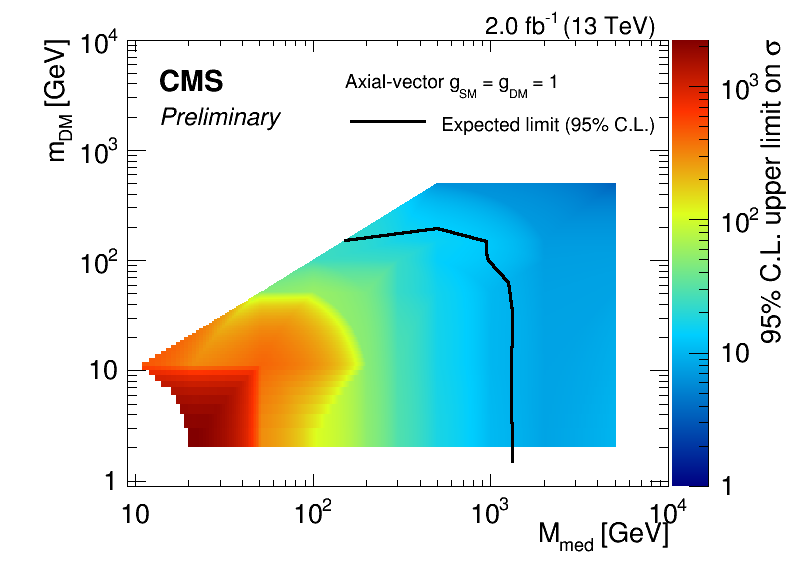
\includegraphics[width=0.75\textwidth]{figures/DMplots/dm_A_g1p0_2p0fb_2dlimits} \\
\caption{Expected 95\% CL upper limit on the cross section, and exclusion
contour for the axial-vector light flavour model with unity couplings at 2~\ifb.}
\label{fig:dm_A_g1_2fb_2dlimits}
\end{center}
\end{figure}

\begin{figure}
\begin{center}
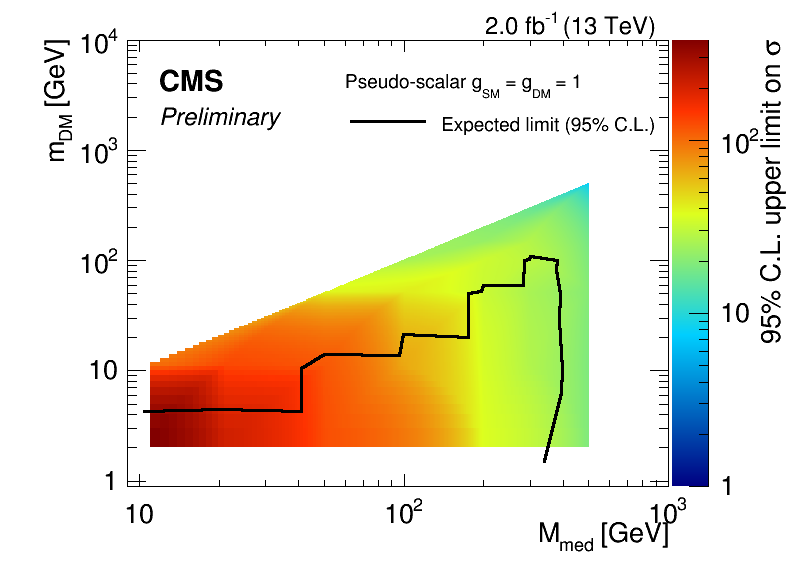
\includegraphics[width=0.75\textwidth]{figures/DMplots/dm_P_g1p0_2p0fb_2dlimits} \\
\caption{Expected 95\% CL upper limit on the cross section, and exclusion
contour for the pseudoscalar light flavour model with unity couplings at 2~\ifb.}
\label{fig:dm_P_g1_2fb_2dlimits}
\end{center}
\end{figure}

\clearpage

\begin{table}
\small
\begin{center}
\caption{Background and signal yields, and signal significance for a vector light jet model point}
\label{tab:MSB_V_g1_2fb}
\begin{tabular}{|l|l|l|l|l|}
\textbf{Vector Mphi-1000 Mchi-50 gSM-1p0 gDM-1p0}   &  bgTtw    &  bgZinv   &  Signal &
Significance \\ 
\hline
htBin 250-300 cat eq1j eq0b mht 0 &     36.75    &  205.88   &  31.90   &0.42 \\ 
htBin 300-350 cat eq1j eq0b mht 0 &     16.52    &  118.02   &  18.35   &0.42 \\ 
htBin 250-300 cat eq2a eq0b mht 250 &   15.77    &  51.84    &  8.99    &0.38 \\ 
htBin 250-300 cat eq3a eq0b mht 225 &   7.59     &  23.80    &  3.84    &0.33 \\ 
htBin 250-300 cat eq3j eq0b mht 0 &     2.80     &  7.88     &  1.59    &0.29 \\ 
\end{tabular}
\end{center}
\end{table}

\begin{table}
\small
\begin{center}
\caption{Background and signal yields, and signal significance for an axial-vector light jet model point}
\label{tab:MSB_A_g1_2fb}
\begin{tabular}{|l|l|l|l|l|}
\textbf{Axial Mphi-1000 Mchi-50 gSM-1p0 gDM-1p0}    &  bgTtw    &  bgZinv   &  Signal &
Significance \\ 
\hline
htBin 300-350 cat eq1j eq0b mht 0 &     16.52    &  118.02   &  15.93   &0.37 \\ 
htBin 250-300 cat eq1j eq0b mht 0 &     36.75    &  205.88   &  28.19   &0.37 \\ 
htBin 250-300 cat eq2j eq0b mht 200 &   11.97    &  37.94    &  5.28    &0.31 \\ 
htBin 200-250 cat eq1j eq0b mht 0 &     102.20   &  480.39   &  46.04   &0.26 \\ 
htBin 200-250 cat eq2a eq0b mht 225 &   13.86    &  42.53    &  5.41    &0.25 \\ 
\end{tabular}
\end{center}
\end{table}

\clearpage

\begin{table}
\small
\begin{center}
\caption{Background and signal yields, and signal significance for a scalar light jet model point}
\label{tab:MSB_S_g1_2fb}
\begin{tabular}{|l|l|l|l|l|}
\textbf{Scalar Mphi-100 Mchi-10 gSM-1p0 gDM-1p0}    &  bgTtw    &  bgZinv   &  Signal &
Significance \\ 
\hline
htBin 200-250 cat eq2a eq0b mht 225 &   13.86    &  42.53    &  1.08    &0.03 \\ 
htBin 200-250 cat eq2a eq0b mht 175 &   48.97    &  128.23   &  1.90    &0.03 \\ 
htBin 200-250 cat eq2a eq1b mht 225 &   1.89     &  3.02     &  0.18    &0.03 \\ 
htBin 200-250 cat eq1j eq0b mht 0 &     102.20   &  480.39   &  6.39    &0.03 \\ 
htBin 350-400 cat ge5a eq0b mht 0 &     2.01     &  5.92     &  0.09    &0.02 \\ 
\end{tabular}
\end{center}
\end{table}

\begin{table}
\small
\begin{center}
\caption{Background and signal yields, and signal significance for a pseudoscalar light jet model point}
\label{tab:MSB_P_g1_2fb}
\begin{tabular}{|l|l|l|l|l|}
\textbf{Pseudoscalar Mphi-100 Mchi-10 gSM-1p0 gDM-1p0}  &  bgTtw    &  bgZinv   &  Signal &
Significance \\ 
\hline
htBin 200-250 cat eq3a eq0b mht 175 &   12.68    &  33.18    &  1.18    &0.07 \\ 
htBin 250-300 cat eq3a eq0b mht 225 &   7.59     &  23.80    &  0.63    &0.06 \\ 
htBin 200-250 cat eq1j eq0b mht 0 &     102.20   &  480.39   &  7.66    &0.04 \\ 
htBin 200-250 cat eq2a eq2b mht 175 &   1.07     &  0.87     &  0.09    &0.04 \\ 
htBin 200-250 cat eq2a eq0b mht 225 &   13.86    &  42.53    &  0.63    &0.03 \\ 
\end{tabular}
\end{center}
\end{table}


\clearpage

%\begin{figure}[h!] \centering
%\subfigure{\includegraphics[width=0.5\textwidth]{figures/DMplots/bla.pdf}}
%\subfigure{\includegraphics[width=0.5\textwidth]{figures/DMplots/bla.pdf}}
%\caption{\label{fig:limits_S} Expected exclusion contours at 95\% CL for
%3\fbinv and 10\fbinv using scalar couplings. } \end{figure}


\clearpage \subsection{Heavy flavour models} \label{sec:dm_heavyjet}

Owing to the principal of Minimal Flavor Violation (MFV), top and bottom quarks
can play important roles in the phenomenology of dark matter. Scalar and
pseudoscalar models predict not only the `monojet' processes described in
Sec.~\ref{sec:dm_lightjet} but also the production of dark matter in association
with top (or bottom) pairs. This results in signatures with relatively large jet
multiplicities, in particular for \DMtt production. The \alphat analysis is well 
suited to searching for such signatures. An example Feynman diagram for the pair
production of dark matter particles in association with pairs of heavy quarks is
shown in Fig.~\ref{fig:feynman_hf}.


\begin{figure}[h!] \centering
\subfigure{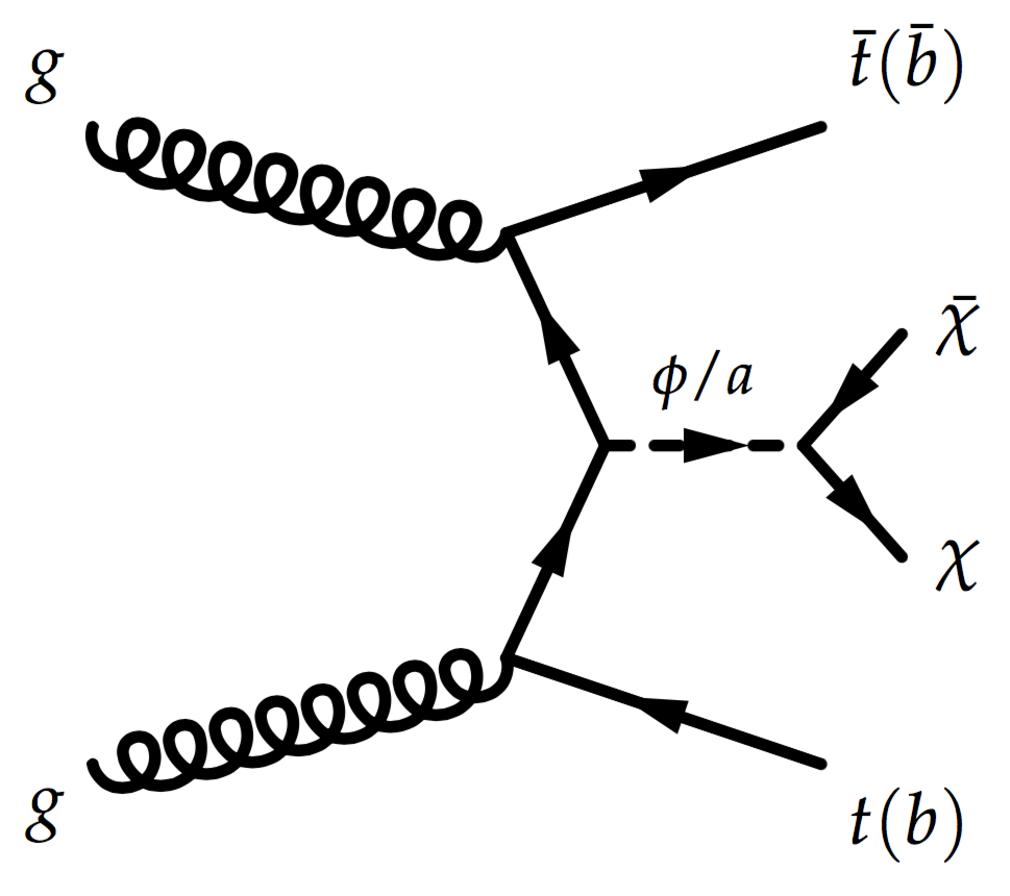
\includegraphics[width=0.35\textwidth]{figures/DMplots/feynman_hf.pdf}}
\caption{Feynman diagram of the pair production of Dark Matter particles in
association with $t\bar{t}$ or $b\bar{b}$. \cite{Abercrombie:2015wmb}}
\label{fig:feynman_hf} \end{figure}


The cross sections, signal yields and efficiencies for scalar and pseudoscalar
\DMtt models expected with 2~\ifb of data are shown in
Tables~\ref{tab:dm_DMttS_2fb}~and~\ref{tab:dm_DMttP_2fb}. The selection
efficiencies for these models are around $\sim 10$\%, and the improvement
provided by the new asymmetric and monojet categories is again evident.

\clearpage 
\begin{table}
\renewcommand{\arraystretch}{1.0}
\small
\centering
\begin{tabular}{lllllll}
\hline
$m_\phi$ & $m_\chi$ & $\sigma$ [pb] & Yield (sym) & Yield (asy) & Yield (mon) & Efficiency [\%] \\ \hline
100       &   10        &   6.73e-01  &   36.36     &   8.16      &   17.63     &   2.70      \\ 
10        &   10        &   9.49e-02  &   2.38      &   0.55      &   1.22      &   1.25      \\ 
50        &   10        &   2.94e+00  &   72.01     &   18.32     &   36.53     &   1.22      \\ 
200       &   150       &   1.30e-04  &   0.03      &   0.01      &   0.02      &   13.16     \\ 
500       &   150       &   3.75e-03  &   1.02      &   0.15      &   0.48      &   13.55     \\ 
1000      &   1         &   3.69e-04  &   0.12      &   0.02      &   0.06      &   15.79     \\ 
100       &   1         &   6.72e-01  &   35.88     &   7.42      &   18.04     &   2.67      \\ 
10        &   1         &   1.96e+01  &   146.33    &   43.66     &   65.49     &   0.37      \\ 
200       &   1         &   9.33e-02  &   13.54     &   2.34      &   6.68      &   7.26      \\ 
20        &   1         &   1.05e+01  &   116.24    &   34.16     &   54.99     &   0.55      \\ 
300       &   1         &   2.95e-02  &   6.33      &   1.02      &   3.09      &   10.72     \\ 
500       &   1         &   5.18e-03  &   1.38      &   0.23      &   0.66      &   13.34     \\ 
50        &   1         &   2.94e+00  &   69.98     &   16.63     &   33.60     &   1.19      \\ 
500       &   500       &   9.89e-07  &   0.00      &   0.00      &   0.00      &   17.51     \\ 
200       &   50        &   9.22e-02  &   13.73     &   2.45      &   6.47      &   7.44      \\ 
300       &   50        &   2.90e-02  &   6.49      &   1.04      &   3.13      &   11.19     \\ 
50        &   50        &   2.33e-03  &   0.29      &   0.06      &   0.14      &   6.29      \\ 
\hline
\end{tabular}
\caption{Cross section, yields at 2~\ifb (split according to symmetric, asymmetric, and monojet categories), and total selection efficiency for the scalar DM$+t\bar{t}$ samples.}
\label{tab:dm_DMttS_2fb}
\end{table}

%\clearpage
\begin{table}
\renewcommand{\arraystretch}{1.0}
\small
\centering
\begin{tabular}{lllllll}
\hline
$m_\phi$ & $m_\chi$ & $\sigma$ [pb] & Yield (sym) & Yield (asy) & Yield (mon) & Efficiency [\%] \\ \hline
100       &   10        &   1.90e-01  &   26.97     &   5.48      &   12.82     &   7.09      \\ 
10        &   10        &   1.50e-02  &   1.88      &   0.39      &   0.94      &   6.28      \\ 
50        &   10        &   3.03e-01  &   34.57     &   8.15      &   16.40     &   5.70      \\ 
200       &   150       &   4.12e-04  &   0.10      &   0.02      &   0.05      &   12.39     \\ 
500       &   150       &   4.61e-03  &   1.22      &   0.21      &   0.60      &   13.18     \\ 
100       &   1         &   1.91e-01  &   27.59     &   6.00      &   12.71     &   7.23      \\ 
10        &   1         &   4.41e-01  &   37.69     &   7.87      &   18.60     &   4.27      \\ 
200       &   1         &   8.36e-02  &   15.86     &   3.26      &   7.69      &   9.48      \\ 
20        &   1         &   3.99e-01  &   36.36     &   8.59      &   17.64     &   4.55      \\ 
300       &   1         &   4.00e-02  &   8.74      &   1.63      &   4.21      &   10.93     \\ 
500       &   1         &   5.41e-03  &   1.39      &   0.24      &   0.66      &   12.87     \\ 
50        &   1         &   3.03e-01  &   35.23     &   7.97      &   17.00     &   5.81      \\ 
500       &   500       &   3.27e-06  &   0.00      &   0.00      &   0.00      &   17.14     \\ 
200       &   50        &   8.38e-02  &   15.95     &   3.33      &   7.67      &   9.51      \\ 
300       &   50        &   3.99e-02  &   8.60      &   1.61      &   4.19      &   10.78     \\ 
50        &   50        &   2.98e-03  &   0.54      &   0.10      &   0.26      &   9.04      \\ 
\hline
\end{tabular}
\caption{Cross section, yields at 2~\ifb (split according to symmetric, asymmetric, and monojet categories), and total selection efficiency for the pseudo-scalar DM$+t\bar{t}$ samples.}
\label{tab:dm_DMttP_2fb}
\end{table}
 
\clearpage


\subsubsection{Projected sensitivities}

The expected 95\% CL signal strength limits for simplified \DMtt models with scalar and
pseudo-scalar couplings are calculated for 2~\ifb. These are shown in
Tables~\ref{tab:dm_DMttS_2fb_limits}~and~\ref{tab:dm_DMttP_2fb_limits}. At this
integrated luminosity, the sensitivity approaches scalar mediator masses of up 
to 100~GeV and DM masses of about 10 GeV, whereas it is insufficient to
significantly exclude the pseudoscalar model, which has generally smaller cross
sections.

Figure~\ref{fig:dm_DMttS_2fb_2dlimits} shows the interpolated scalar expected 
exclusion contour in the {\mphi-\mchi} mass plane.

Tables~\ref{tab:MSB_DMttS_2fb} and \ref{tab:MSB_DMttP_2fb} summarise the most sensitive 
{(\njet,\nb,\scalht,\mht)} signal region
bins for a representative mass point (near the exclusion boundary) of each \DMtt
model. As expected, the sensitivity for these models mostly lies at large jet and b-jet
multiplicities, medium-high \scalht, and at \mht values closer to the lower bound
of the relevant \scalht bin. Note that, for convenience, all signal models have
been normalised to a cross section of 10 pb in these tables.


\clearpage
\begin{table}
\renewcommand{\arraystretch}{2.0}
\begin{center}
\caption{95\% CL upper limits on the signal strength at 2~\ifb for the scalar DM$+t\bar{t}$ samples}
\label{tab:dm_DMttS_2fb_limits}
\begin{tabular}{lccccccccc}
\multirow{5}{*}{\rotatebox{90}{$m_{\rm{DM}}$ (GeV)}}
& \multicolumn{1}{c|}{500} &  &  &  &  &  &  & 9.38e+04 & \\ 
& \multicolumn{1}{c|}{150} &  &  &  &  & 1.16e+03 &  & 40.32 & \\ 
& \multicolumn{1}{c|}{50} &  &  & 153.05 &  & 3.33 & 6.90 &  & \\ 
& \multicolumn{1}{c|}{10} & 16.01 &  & 0.53 & 1.17 &  &  &  & \\ 
& \multicolumn{1}{c|}{1} & 0.25 & 0.33 & 0.54 & 1.29 & 3.40 & 7.12 & 31.11 & 331.08\\ 
\cline{2-10}
& \multicolumn{1}{c|}{} & 10 & 20 & 50 & 100 & 200 & 300 & 500 & 1000\\ 
& & \multicolumn{7}{c}{$M_{\rm{Med}}$ (GeV)}
\end{tabular}
\end{center}
\end{table}

\begin{table}
\renewcommand{\arraystretch}{2.0}
\begin{center}
\caption{95\% CL upper limits on the signal strength for 2.1~\ifb for the pseudo-scalar DM$+t\bar{t}$ samples}
\begin{tabular}{lcccccccc}
\label{tab:dm_DMttP_2fb_limits}
\multirow{5}{*}{\rotatebox{90}{$m_{\rm{DM}}$ (GeV)}}
& \multicolumn{1}{c|}{500} &  &  &  &  &  &  & 2.83e+04\\ 
& \multicolumn{1}{c|}{150} &  &  &  &  & 414.40 &  & 32.83\\ 
& \multicolumn{1}{c|}{50} &  &  & 80.31 &  & 2.74 & 5.02 & \\ 
& \multicolumn{1}{c|}{10} & 23.13 &  & 1.27 & 1.67 &  &  & \\ 
& \multicolumn{1}{c|}{1} & 1.16 & 1.21 & 1.24 & 1.56 & 2.75 & 4.76 & 29.80\\ 
\cline{2-9}
& \multicolumn{1}{c|}{} & 10 & 20 & 50 & 100 & 200 & 300 & 500\\ 
& & \multicolumn{6}{c}{$M_{\rm{Med}}$ (GeV)}
\end{tabular}
\end{center}
\end{table}

\clearpage

\begin{figure}
\begin{center}
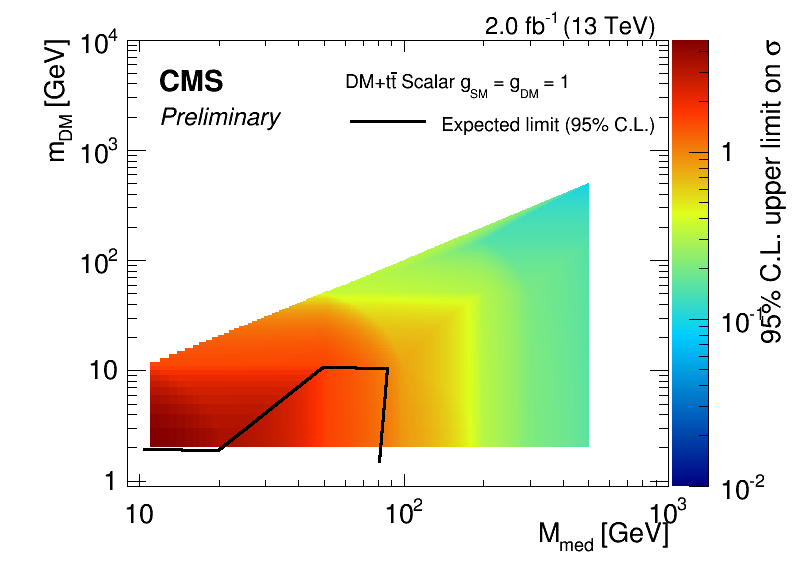
\includegraphics[width=0.75\textwidth]{figures/DMplots/dm_DMttS_2p0fb_2dlimits} \\
\caption{Expected 95\% CL upper limit on the cross section, and exclusion
contour for the scalar \DMtt model with unity couplings at 2~\ifb.}
\label{fig:dm_DMttS_2fb_2dlimits}
\end{center}
\end{figure}

\clearpage

\begin{table}
\small
\begin{center}
\caption{Background and signal yields, and signal significance for a scalar \DMtt model point}
\label{tab:MSB_DMttS_2fb}
\begin{tabular}{|l|l|l|l|l|}
\textbf{TTbarDMJets scalar Mchi-10 Mphi-100 25ns mht}    &  bgTtw    &  bgZinv   &  Signal &     Significance \\ 
\hline
htBin 400-500 cat ge5a eq2b mht 0 &     0.65     &  0.69     &  11.76   &7.88 \\ 
htBin 400-500 cat ge5a eq1b mht 150 &   1.77     &  2.77     &  15.81   &6.12 \\ 
htBin 300-350 cat eq4a eq1b mht 175 &   2.53     &  2.24     &  13.79   &5.10 \\ 
htBin 400-500 cat ge5j eq1b mht 150 &   1.69     &  3.89     &  14.60   &5.00 \\ 
htBin 350-400 cat ge5a eq2b mht 0 &     0.53     &  0.23     &  6.89    &4.67 \\ 
\end{tabular}
\end{center}
\end{table}

\begin{table}
\small
\begin{center}
\caption{Background and signal yields, and signal significance for a pseudoscalar \DMtt jet model point}
\label{tab:MSB_DMttP_2fb}
\begin{tabular}{|l|l|l|l|l|}
\textbf{TTbarDMJets pseudoscalar Mchi-10 Mphi-100 25ns mht}  &  bgTtw    &  bgZinv   &  Signal &     Significance \\ 
\hline
htBin 500-600 cat ge5j eq2b mht 225 &   0.39     &  1.03     &  28.23   &18.36 \\ 
htBin 350-400 cat ge5a eq1b mht 0 &     1.23     &  1.12     &  30.25   &16.90 \\ 
htBin 400-500 cat ge5a eq1b mht 150 &   1.77     &  2.77     &  42.35   &16.42 \\ 
htBin 400-500 cat ge5a eq2b mht 0 &     0.65     &  0.69     &  23.80   &15.98 \\ 
htBin 400-500 cat ge5j eq2b mht 150 &   0.69     &  0.67     &  24.60   &15.88 \\ 
\end{tabular}
\end{center}
\end{table}


